% \documentclass[sigconf,anonymous, review]{aamas}
\documentclass[runningheads]{llncs}
\newcommand{\mps}[1]{\textbf{M: \textcolor{green}{#1}}\newline}
\usepackage{balance}
\usepackage{tikz}
\usepackage{listings}
\usepackage{xcolor}
\usepackage{xspace}
\colorlet{brightlightbluegray}{red!9!green!8!blue!6}%
\colorlet{redgb}{red!91!green!92!blue!94}%
\colorlet{rgreenb}{green!70!black}%
\colorlet{rgblue}{red!20!green!20!blue!94}%
% \colorlet{darkbluegray}{blue!20!gray!80}%
\colorlet{mediumbluegray}{blue!20!gray!40}%
\usetikzlibrary{arrows.meta, positioning, shapes.geometric}

% \setcopyright{ifaamas}
% \acmConference[AAMAS '26]{Proc.\@ of the 25th International Conference
% on Autonomous Agents and Multiagent Systems (AAMAS 2026)}{May 25 -- 29, 2026}
% {Paphos, Cyprus}{C.~Amato, L.~Dennis, V.~Mascardi, J.~Thangarajah (eds.)}
% \copyrightyear{2026}
% \acmYear{2026}
% \acmDOI{}
% \acmPrice{}
% \acmISBN{}

% \acmSubmissionID{<<submission id>>}

\newcounter{mpscount}
\newcounter{akccount}
\newcounter{shccount}
\newcounter{ojcount}
\DeclareRobustCommand{\mps}[1]{\stepcounter{mpscount}\textcolor{blue!60!black}{\textsf{MPS \thempscount: #1}}}
\DeclareRobustCommand{\akc}[1]{\stepcounter{akccount}\textcolor{red}{\textsf{AKC \theakccount: #1}}}
\newcommand{\oj}[1]{\stepcounter{ojcount}\textcolor{green!60!black}{\textsf{OJ \theojcount: #1}\newline}}

\lstset{
    basicstyle=\small\ttfamily,
    breaklines=true,
    frame=single,
    xleftmargin=15pt,
    xrightmargin=5pt,
    rulecolor=\color{gray!50},
    backgroundcolor=\color{gray!5},
}

\newcommand{\ahoy}{Ahoy\xspace}

\usepackage{soul}

% \title{Coordinated Heterogeneous Intelligent Protocol Selection: {\ahoy}}

% \author{Omkar Joshi}
% \affiliation{
%   \institution{North Carolina State University}
%   \city{Raleigh}
%   \country{USA}}
% \email{ojjoshi@ncsu.edu}

% \author{Nimue}
% \affiliation{
%   \institution{The Lady's Lake}
%   \city{Avalon}
%   \country{United Kingdom}}
% \email{lady.of.the.lake@avalon.uk}

\begin{document}
%
\title{\ahoy: LLMs Enacting Multiagent Interaction Protocols}
%
\titlerunning{\ahoy}

\author{Omkar Joshi\inst{1}\orcidID{0009-0006-5069-2326} \and
Amit K. Chopra\inst{2}\orcidID{0000-0003-4629-7594} \and
Munindar P. Singh\inst{1}\orcidID{0000-0003-3599-3893}}
%
\authorrunning{O. Joshi et al.}

\institute{North Carolina State University, Raleigh, NC, USA \and
Lancaster University, Lancaster, UK }

\maketitle

\mps{* refers to my advice pages}

\mps{G refers to grammar}

\begin{abstract}
Multiagent systems typically require protocol-specific agent implementations: a change in the protocol necessitates different agents or extensive code modifications.
This tight coupling makes it difficult to build flexible agents.
We demonstrate that \emph{Large Language Models} can overcome this limitation by enabling a single agent to correctly enact multiple protocols without protocol-specific engineering.
We introduce \emph{\ahoy}, an approach that enables LLM-driven agents to select and enact multiple interaction protocols guided by natural language input from users. 
\ahoy creates agents that are protocol-agnostic --- operating without protocol-specific code --- while respecting BSPL protocol constraints that ensure correct behavior.
Our key contribution is a generic agent adapter ({\ahoy}) that decouples agent decision making from protocol specification. 
We evaluate \ahoy across two distinct protocols---Logistics (packaging and shipping coordination) and Purchase (buyer-seller-shipper coordination).
% \akc{not sure whether LLM time by itself matters. if it were relativized to something protocol-related, e.g., number of enabled messages inspected, length of enactment, then perhaps we could make a scalability argument}

Our results show that \ahoy-enabled LLMs correctly select and enact protocols without specialized training, producing no adapter exceptions, malformed messages, or constraint violations.
\ahoy also supports the construction of agents that can intelligently exploit flexible protocols.
This approach reduces knowledge engineering overhead by enabling agents to participate in multiple protocols, demonstrating how LLM--enabled multiprotocol architectures enable adaptive coordination in evolving business domains, addressing a key challenge for scaling multiagent systems. 

% \mps{the keywords shouldn't overlap with the title}

\end{abstract}

\keywords{Multiagent Systems}

%%%%%%%%%%%%%%%%%%%%%%%%%%%%%%%%%%%%%%%%%%%%%%%%%%%%%%%%%%%%%%%%%%%%%%%%%%%%%%%%%%%
\section{Introduction}\label{Introduction}
Agentic AI is the idea that \ldots.  The promise of agentic AI is \ldots

Agentic AI is a multiagent enterprise. Agent interaction protocols are therefore crucial.  Several protocols have been proposed to support agent interaction, e.g., A2A.  They have limitations...

A major limitation of the traditional approach to MAS is that execution of new protocols require the development of new agents.

% The information protocols paradigm. Decentralized, asynchronous. Several programming models for agents have been proposed, enabling the creation of ``rule-based'' agents in Python and BDI. 

Recent advances in generative AI have led to the development of Large Language Models that demonstrate reasoning ability.

An LLM agent is \ldots
We investigate the possibility of whether LLM agent may execute information protocols correctly and in a manner that aligns with its user's goals. 

% We contribute a protocol-based programming model for LLM agents. We demonstrate that LLM agents are able to judiciously (in line with user goals) execute protocols.

% We leave user dialog as out of scope.


% \begin{itemize}
%     \item What are protocols?
%     \item Biggest problem with agents is that we need to trade off generalizability with task-specific performance.
%     \item An agent that can participate in multiple protocols based on user requirements is useful.
%     \item The user interacts with the agent via natural language only (no code changes), which simplifies the programming model.
% \end{itemize}

Research Question:
\textit{Can LLM agents effectively select and execute multiple protocols without protocol-specific training or fine-tuning?}

Our key contributions are as follows:
\begin{itemize}
    \item A multiprotocol selection framework to detect appropriate protocol based on natural language input.
    \item A generic agent implementation ({\ahoy}) that can participate in multiple protocols with minimal code changes.
    \item Empirical Evaluation across two/three protocols\\
    \oj{subject to time constraint}
\end{itemize}

%%%%%%%%%%%%%%%%%%%%%%%%%%%%%%%%%%%%%%%%%%%%%%%%%%%%%%%%%%%%%%%%%%%%%%%%%%%%%%
\section{Background}\label{sec:Background}

\subsection{Multiagent Coordination --- Specifying Interaction Protocols}
Formally specified rules of encounter, e.g., in BSPL, define the messages, roles, and constraints that guide agent interactions.
Traditional approaches require agent implementations to be fixed at design time and changes in the requirement or protocol require agent--level code changes.\\
\emph{BSPL} (Blindingly Simple Protocol Language) is a declarative specification language where protocols are described in terms of roles, messages, and logical constraints. 
\oj{add bspl explanation}\oj{add bspl protocol example}

\subsection{Programming Agents Based on Interaction Protocols}

Kiko is a framework for implementing protocol-based agents. 
It provides an adapter that exposes a Python API based on decorators for implementing agents. 
The API allows developers to plug in the agent's reasoning (e.g. when to take an action or send messages), while the adapter handles prototol compliance.\\
\oj{enhance kiko explanation}\oj{insert Kiko example here}



\subsection{Programming LLM Agents}
Large Language Models can be used as the reasoning component in agent architectures.
Programming LLM agents typically involves:
\begin{itemize}
    \item System Prompts
    \item User Prompts
    \item Tool Calling
    \item Memory (RAG/Agent Notes)
\end{itemize}
These components work together to create an agentic loop where the LLM observes state, reasons about options and takes actions.\\
\oj{Enhance the programming components descriptions}\oj{Add a simple example of LLM programming here}

%%%%%%%%%%%%%%%%%%%%%%%%%%%%%%%%%%%%%%%%%%%%%%%%%%%%%%%%%%%%%%%%%%%%%%%%%%%%%%%%
\section{Architecture}

\ahoy achieves protocol agnosticism by decoupling LLM reasoning from protocol-specific logic. 
Rather than implementing distinct agents for each protocol, \ahoy uses a unified architecture where the LLM serves as the decision-making layer, reasoning over constraints and possibilities defined by BSPL protocols.
The architecture orchestrates interaction between four key components through a well-defined flow:

\begin{enumerate}
    \item \textbf{Initialization Phase (One-Time):} When a user provides a natural language goal, the \emph{role detection module} (part of the LLM decision layer) queries the LLM to select an appropriate protocol and role from available options. This selection is fixed for the lifetime of the agent instance. Once the protocol and role are determined, a Kiko adapter is instantiated for that specific protocol-role pair, and the prompt construction layer generates a system prompt containing foundational knowledge about BSPL semantics and the selected protocol.
    
    \item \textbf{Execution Loop (Repeated):} During protocol enactment, the Kiko adapter monitors protocol state and triggers a decision event whenever state changes (e.g., a message arrives from another agent or a custom event fires). The decision endpoint (mediator between LLM and adapters) receives this event and invokes the prompt construction layer to assemble a context-aware user prompt from the current adapter state. The user prompt is passed to the \emph{message decision module} (part of the LLM decision layer), which selects which enabled message to send and how to bind its parameters. The decision endpoint returns this choice to the adapter, which validates and sends the message.
    
    \item \textbf{Termination Check (Each Iteration):} Before each new decision, the \emph{termination condition detection module} (part of the LLM decision layer) checks whether the protocol should conclude. Termination can result from either protocol-driven completion (adapter detects terminal state) or user-defined criteria (e.g., threshold met, timeout reached). If termination conditions are satisfied, the protocol enactment concludes and the adapter shuts down gracefully.
    
    \item \textbf{Concurrency (Optional):} Multiple Kiko adapters can execute concurrently, each managing isolated social state for a different protocol instance. The decision endpoint can interleave decisions across adapters, with the LLM receiving distinct prompts for each protocol context.
\end{enumerate}

This design separates concerns across four layers: the LLM decision layer handles all reasoning (protocol selection, termination detection, message choice), the prompt construction layer transforms protocol state into LLM input, the decision endpoint orchestrates communication flow, and the Kiko adapters enforce all structural constraints and manage protocol state. 
This separation enables protocol agnosticism: new protocols require only a new BSPL specification file, not new LLM logic.
The architecture is illustrated in Figure \ref{fig:architecture_diagram}.
The remainder of this section details each component's role in this flow.

\begin{figure*}[ht]
    \centering
    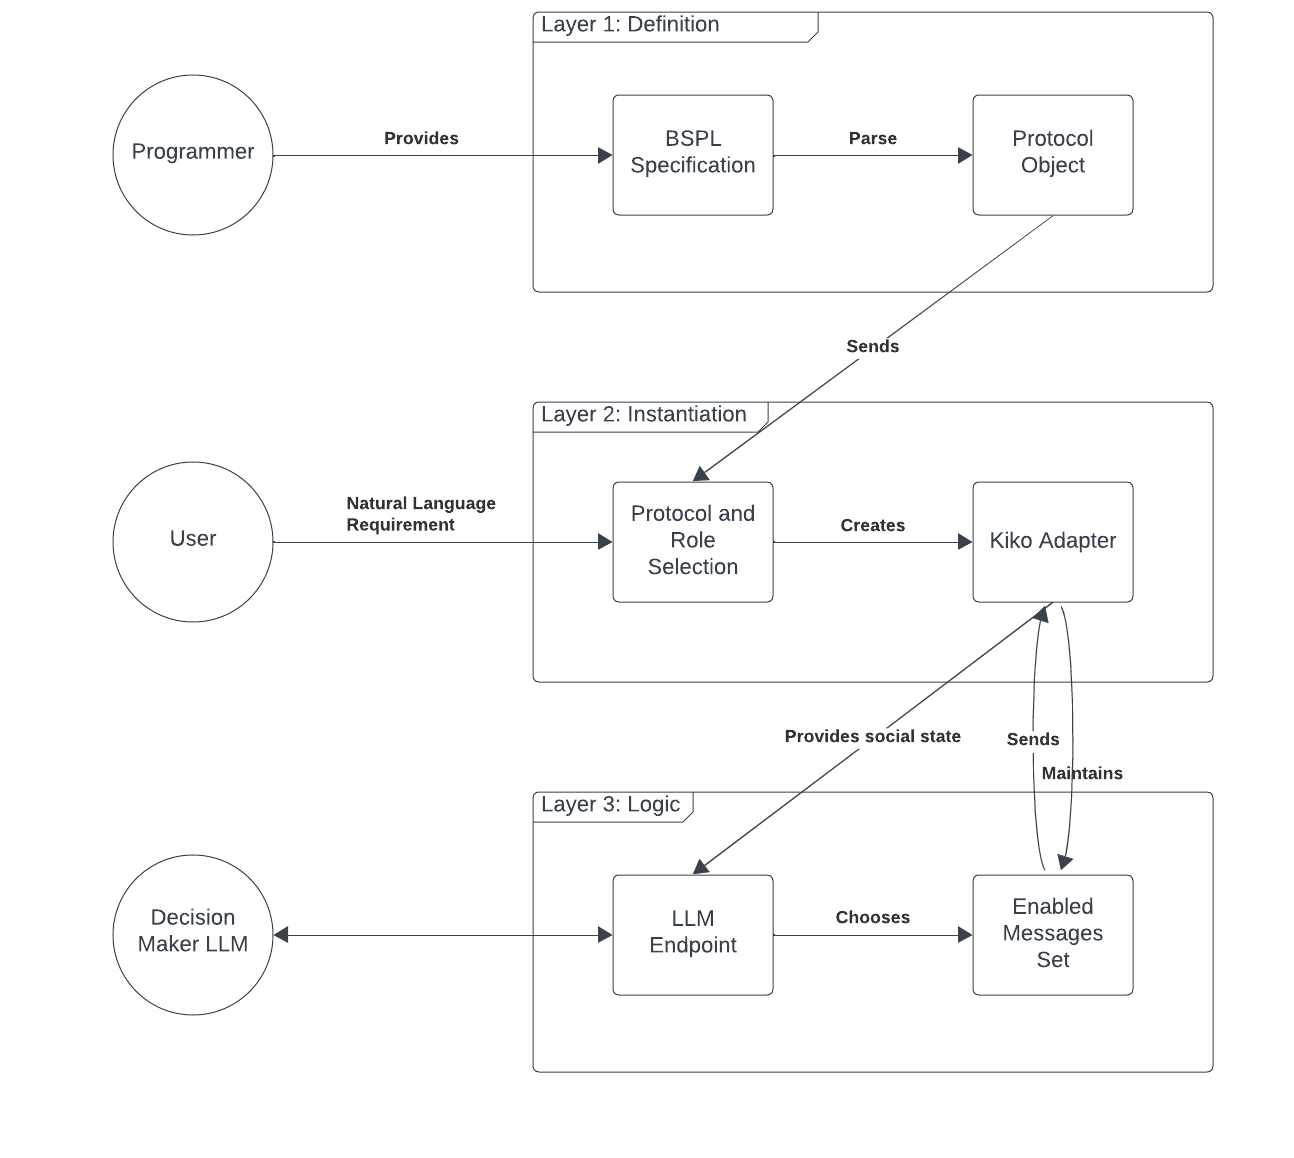
\includegraphics[width=\textwidth]{Images/Architecture Diagram.png}
    \caption{{\ahoy} Architecture Overview}
    \label{fig:architecture_diagram}
\end{figure*}

\subsection{LLM Decision Layer}

The LLM decision layer is responsible for all reasoning about protocol selection and execution. 
It consists of three interdependent modules that operate in sequence during agent initialization and execution.

\subsubsection{Role Detection Module}
The role detection module determines which protocol and role combination is appropriate for a given user intent. 
When an agent is initialized with a natural language goal (e.g., ``I want to buy a notebook''), this module queries the LLM with the set of available protocols, their roles, and the user goal. 
The LLM selects the protocol-role pair that best aligns with the stated objective. 
This determination happens once during initialization and is then fixed for the lifetime of that agent instance, ensuring consistent role behavior throughout execution.

\subsubsection{Termination Condition Detection Module}
The termination condition detection module monitors whether a protocol enactment should conclude. 
Termination can occur for two reasons: (1) the protocol reaches a terminal state (successful completion or deadlock detected by the Kiko adapter), or (2) user-defined termination criteria are met (e.g., a transaction value exceeds a threshold, a timeout is reached, or a satisfaction condition is met). 
This module queries the current protocol state, consults any external conditions or alerts, and signals the adapter to halt gracefully when appropriate. 
By separating termination detection from the message decision logic, \ahoy can handle both protocol-driven and domain-driven conclusion criteria.

\subsubsection{Message Decision and Parameter Binding Module}
The message decision module is the core reasoning component that executes repeatedly during protocol enactment. 
When a decision event is triggered (either by an incoming message or a custom event), this module receives: (1) the set of enabled messages from the Kiko adapter (all messages that can legally be sent without violating protocol constraints), (2) the current message history and bound parameters, and (3) agent goals and domain-specific preferences. 
The LLM evaluates the enabled options and selects the message(s) to send along with appropriate parameter bindings. 
The module is constrained to choose only from the enabled message set; the Kiko adapter ensures the preconditions are met, so the LLM need only reason about domain appropriateness and goal alignment.

\subsection{Prompt Construction Layer}

The prompt construction layer transforms protocol state into structured, context-aware LLM input. 
Prompts are assembled in two phases: a static system prompt constructed once per protocol enactment, and dynamic user prompts constructed on each decision event.

\subsubsection{System Prompt}
The system prompt, created once when the protocol and role are determined, establishes foundational knowledge that persists across all decision iterations. 
It contains: (1) an explanation of BSPL semantics (roles, messages, parameter binding rules), (2) the agent's assigned role and protocol, (3) an explanation of enabled messages and how constraints work, (4) available tools and their calling conventions, and (5) human-readable guidelines for parameter binding. 
The system prompt is cached and reused to minimize API calls and maintain consistency. 
It is overwritten only when a new protocol enactment begins.

\subsubsection{User Prompt}
For each decision event, a fresh user prompt is constructed by querying the Kiko adapter for current state. 
The user prompt is assembled from: (1) a role reminder establishing the agent identity and decision task, (2) the complete message history from the adapter showing all messages sent and received, (3) currently enabled messages extracted from the adapter's enabled message store, (4) bound parameters already set by prior messages, and (5) which parameters must be filled for each enabled message option. 
This prompt encodes sufficient context for the LLM to make informed decisions while remaining concise enough to stay within token limits.

\subsection{Decision Endpoint}

The decision endpoint is an event handler that mediates between the Kiko adapter and the LLM decision layer. 
It is registered as a callback with the adapter and triggered whenever protocol state changes. 
The decision endpoint executes the following sequence: (1) receive a trigger event (message received, custom timeout fired, etc.) from the adapter, (2) invoke the termination detection module to check if the protocol should conclude, (3) if not terminating, construct the user prompt from current adapter state, (4) call the LLM decision module with the assembled system and user prompts, (5) parse the LLM's response to extract selected message type and parameter bindings, (6) return the selected message instance to the adapter, which sends it according to protocol constraints. 
Because the adapter enforces all structural constraints, the decision endpoint can focus purely on domain reasoning without duplicating validation logic. 
This separation of concerns is the key to protocol agnosticism: the same endpoint logic works for any protocol.

\subsection{Kiko Adapters ($n$ Instances)}

\ahoy instantiates one Kiko adapter per protocol-role pair being executed. 
Each adapter is independent and maintains isolated social state, ensuring that concurrent protocol enactments do not interfere.

\subsubsection{Adapter Responsibilities}
Each Kiko adapter is responsible for: (1) enforcing protocol constraints (message schema validation, precondition checking, state machine transitions), (2) tracking message history and parameter bindings in isolated social state, (3) computing the set of enabled messages at each step (all messages whose preconditions are satisfied), (4) sending and receiving messages according to protocol rules, (5) detecting protocol terminal states (completion or deadlock), and (6) invoking registered decision endpoint callbacks when state changes. 
The adapter provides a Python API (via decorators such as \texttt{@adapter.reaction(MessageType)}) that allows agents to register handlers for protocol events.

\subsubsection{Social State Isolation}
Because each protocol instance has its own adapter, parameters are naturally scoped per protocol. 
For example, an \texttt{orderID} parameter in the Purchase protocol is isolated from an \texttt{orderID} in the Logistics protocol; they do not interfere even though they share the same name. 
This isolation is enforced at the adapter level and requires no special logic in the LLM layer. 
Message history is similarly isolated: the LLM receives only the message history relevant to the current protocol when constructing user prompts.

\subsubsection{Concurrent Execution}
Multiple adapters can run concurrently, enabling a single LLM-driven agent to participate in multiple protocol enactments simultaneously. 
Each adapter maintains its own decision endpoint callback and triggers decisions independently. 
The LLM receives distinct prompts for each protocol context and reasons appropriately for each. 
Concurrency is managed via asynchronous I/O (\texttt{asyncio}) to prevent blocking between protocol instances.


% The {\ahoy} framework can broadly be divided into two parts: a protocol and role selection module, which determines the appropriate combination of role and protocol based on user input; and a generic {\ahoy} agent that performs any role in a multiagent system without code modifications.
% This behavior is enabled by the Kiko adapter, which maintains the social state of the multiagent system and handles sending and receiving messages.
% The {\ahoy} agent extracts the social state of the system using this adapter and queries an external LLM with relevant context (a filtered subset of the social state) and the enabled message options.
% The {\ahoy} agent interacts with the LLM using a structured prompting approach that we describe in greater detail in Section \ref{sec:prompt_construction}.
% Our framework also allows the {\ahoy} agent to access external tools such as a UID generator and agent memory save or edit functions that are independent of the Kiko adapter, further enhancing the framework's flexibility and extensibility.


% \subsection{Component Overview}
% {\ahoy} consists of three key components.

% \subsubsection{Protocol Selection}
% The input to the protocol selection module is the natural language user input and a list of available protocols and roles.
% We then ask the LLM to choose a specific role and protocol from this list that allows the {\ahoy}--enabled agent to fulfill the user intent.
% The output returned by the LLM is then used to instantiate the appropriate Kiko adapter for the selected role and protocol.

% \subsubsection{Generic Agent Adapter}
% {\ahoy} constructs the \emph{system prompt} once during initialization, based on the selected protocol and role.
% This system prompt establishes the LLM's understanding of BSPL semantics, enabled messages and parameter binding rules.
% The system prompt is cached and reused for all subsequent interactions. 
% The construction process is detailed in Section \ref{sec:prompt_construction}. 

% \akc{Seems to me a needless limitation that the only events that can be handled are communication events. I remember you had some technical difficulties earlier in having the LLM invoke adapter functionality; maybe now you have a better grasp of LLM programming?}
% \oj{We shoule be able to handle custom events in the implementation right now. I was just facing issues with how to effectively test them. I have to dig into the Kiko documentation to set up a proper test with custom events.}

% An \ahoy agent then executes the following decision loop:
% \begin{enumerate}
%     \item[Step 1:] \akc{If you need to say Step 1:, what's the point of the LaTeX enumeration?} The Kiko adapter fires the decision event. 
%     \item[Step 2:] The \ahoy \emph{handler} receives the set of enabled messages from the adapter.
%     \item[Step 3:] \ahoy queries the LLM to select one or more enabled messages and bind their parameters.
%     \item[Step 4:] \ahoy returns the selected message instance(s) to the Kiko adapter, which sends them automatically.
%     \item[Step 5:] The loop repeats until the protocol reaches a terminal state (completion or deadlock).
% \end{enumerate}

% \subsubsection{Protocol Adapters}
% The protocol adapter is instantiated at runtime for the selected protocol and role.
% The framework loads the protocol and role objects from the configuration system, instantiates an adapter from the BSPL library and registers the LLM decision handler as a callback.
% The adapter is responsible for maintaining the isolated social state store per agent instance and protocol.
% The adapter also enforces all BSPL rules: precondition checking, state machine transitions, message validation, etc.
% In addition to this, the adapter handles sending and receiving messages.
% When the social state changes and new messages become enabled, the adapter automatically triggers the registered decision handler.

% % \subsubsection{State Store} 
% % The adapter-maintained state store provides the system with per-protocol, per-agent-instance isolation \akc{if this is automatically done by the protocol adapter, then no need for a separate section}.
% % Parameters are scoped per protocol, which means that a parameter named \texttt{orderID} in the Logistics protocol does not interfere with a parameter named \texttt{orderID} in the Purchase protocol.
% % This prevents cross-protocol contamination and allows the framework to provide consistency guarantees \akc{don't get it; likely doesn't belong in this paper}.
% % Since access to this store is allowed only through deterministic adapter methods and not direct LLM calls, we prevent context overload and maintain social state consistency \akc{don't get it}.

% \subsection{Prompt Construction Methodology}\label{sec:prompt_construction}
% \oj{still working on this section, haven't gone over it since I'm planning to rewrite it.}
% We employ a three--stage prompt construction strategy, combining static template strings with content from the current social state to create context-aware prompts for protocol selection and agent decision--making.

% \subsubsection{Protocol Selection Prompt Construction}
% The purpose of the protocol selection prompt is to detect which protocol and role the user needs the {\ahoy} agent to participate in based on natural language input.
% We construct the protocol detection prompt by assembling a task definition, a list of available roles and protocols, and optional disambiguation rules.
% The task definition string prompts the LLM to choose a protocol and role based on the user input, which is taken directly from \texttt{input.txt}.
% The protocol selection module then queries the configuration system to extract protocol information.
% It then iterates over the protocols loaded from \texttt{configuration.py} to create a protocol registry string that contains the protocols and roles available to choose from.
% A sample specification string is shown in Listing \ref{lst:protocol-registry}
% \begin{lstlisting}[language=python, caption={Sample Protocol Summary String}, label={lst:protocol-registry}]
% Available Protocols:

% Logistics: roles [Merchant, Wrapper, Labeler, Packer]
% Purchase: roles [Buyer, Seller, Shipper]
% \end{lstlisting}
% Since this registry string is generated every time the protocol selection module is called, new protocols are automatically included in the protocol selection prompt when the corresponding \texttt{.bspl} file is included the \texttt{/Protocols} folder.
% The CHIPS module also has support to add optional disambiguation rules that can be applied in cases where the information is insufficient for the LLM to make a decision.
% Finally, the output formatting string enforces the response format to be a simple tuple of role and protocol with no additional explanations.
% We then use our validation function (\texttt{validate\_protocol\_and\_role()}) to confirm that the LLM's response maps to an actual protocol and role in the configuration system.
% If invalid, the CHIPS module requests clarification from the user.

% \subsubsection{{\ahoy} System Prompt Construction}
% After selecting the protocol and role, the system prompt is created once and cached for all subsequent decisions in the enactment of that protocol.
% We use a custom BSPL explanation string, shown in Listing \ref{lst:bspl-expl}, which provides a high--level explanation of the BSPL world.
% \begin{lstlisting}[caption=BSPL Explanation String,label=lst:bspl-expl]
% You are participating in BSPL (Blindingly Simple Protocol Language) protocol enactments. 
%     BSPL defines multi-agent protocols where:
%     - Roles are named agents (e.g., Merchant, Buyer)
%     - Messages are directed communication between roles with parameters marked as `out` (sender provides) or `in` (requires prior binding from other messages)
%     - Parameters marked `key` identify protocol instances
%     - You play one role and must track received messages to determine which messages you can legally send next
%     - A message can only be sent when all its `in` parameters are bound by prior messages
%     - When multiple messages are enabled, choose based on domain reasoning and the protocol's intended flow
% \end{lstlisting}
% This string provides foundational BSPL semantics, establishing core concepts (roles, messages, parameters, binding constraints) so the LLM does not need to learn protocol mechanics from scratch.
% We then append an option selection message (Listing \ref{lst:option-selection}) that explains how parameter binding works
% \begin{lstlisting}[language=python, caption={Option Selection String}, label={lst:option-selection}]
% Your choice will directly determine what message gets SENT and what
% happens next:

% The BOUND parameters shown above (in [BOUND: ...]) are already set
% and will be used
% You only need to provide values for parameters marked in FILL ONLY
% Your selection will trigger protocol actions based on the message
% type and parameters
% \end{lstlisting}
% Finally, we append an optional tool specification that documents the available tools and their usage patterns.
% The assembled prompt is cached for reuse.

% \subsubsection{{\ahoy} User Prompt Construction}
% For each decision step, a fresh user prompt is constructed by querying the adapter for the current state and enabled messages.
% {\ahoy} assembles this prompt from multiple components:
% \begin{itemize}
%     \item Agent Role Reminder: This establishes the agent's identity and the decision task. Placeholders are extracted from the social state. (Listing \ref{lst:agent-reminder})
%     \item Message History: This string is dynamically generated by iterating through the messages in the adapter's social state, displaying sender, recipients, message type, and payload parameters. This summarizes information that an intelligent agent is expected to know. (Listing \ref{lst:message-history-generated})
%     \item Enabled Options: This presents the options that the LLM has to choose between. It is extracted from the enabled messages store that the BSPL adapter maintains. (Listing \ref{lst:enabled-options-generated})
%     \item Tool Documentation: This is an optional reminder that contains the information required to call tools.
%     \item Response Format: This is used to enforce the output format to make the LLM response compatible with the parser.
% \end{itemize}

% \begin{lstlisting}[language=python, caption={Agent Role Reminder String}, label={lst:agent-reminder}]
% You are agent '[agent_name]'. Choose at most one option, or return null.
% Your role requires making decisions. When choosing an option, always
% provide values for all required parameters.

% Roles: [Merchant, Wrapper, Labeler, Packer]
% \end{lstlisting}

% \begin{lstlisting}[language=python, caption={Message History String}, label={lst:message-history-generated}]
% === MESSAGE HISTORY ===

% RequestLabel (from Merchant to Wrapper)
% orderID: ORD-001
% address: Warehouse 1

% RequestWrapping (from Wrapper to Merchant)
% orderID: ORD-001
% itemID: ITEM-001

% Label (from Labeler to Merchant)
% itemID: ITEM-001
% labelID: LBL-001

% === END HISTORY (3 messages) ===
% \end{lstlisting}

% \begin{lstlisting}[language=python, caption={Enabled Options String}, label={lst:enabled-options-generated}]
% Options:

% Logistics/RequestWrapping [BOUND: orderID=ORD-001] - FILL ONLY: ['itemID']

% Logistics/Label [BOUND: itemID=ITEM-001] - FILL ONLY: ['labelID']

% Logistics/PackOrder [BOUND: orderID=ORD-001] - FILL ONLY: []
% \end{lstlisting}

% \oj{Include the system architecture diagram}

% The three-stage dynamic prompt generation enables CHIPS {\ahoy}'s core innovation: Protocol Agnostic decision making constrained within the BSPL world.
% The architecture decouples agent implementation from protocol specification.
%  The generic {\ahoy} agent contains no protocol-specific logic that needs to be modified.
% {\ahoy} simply queries the adapter for enabled messages, consults the LLM in a structured and reportable manner, and sends the chosen message.
% All protocol-specific logic is encoded in the BSPL definitions and enforced by the adapter's state machine.
% New protocols only require a new BSPL specification and a user requirement file.
%  This allows the architecture to be scalable across new protocols and use cases and reduces engineering overhead when coordinating across diverse business processes.

%%%%%%%%%%%%%%%%%%%%%%%%%%%%%%%%%%%%%%%%%%%%%%%%%%%%%%%%%%%%%%%%%%%%%%%%%%%%%%%%%%
\section{Programming Model}
% {\ahoy} requires the programmer to provide a protocol specification that defines the messages to be sent, the roles to be performed, and the parameters that need to be bound.\\
% The programmer then interacts with the generic LLM agent using natural language that determines which role the agent needs to play for each enactment.
% \begin{figure*}[ht]
%     \centering
%     \caption{{\ahoy} Agent Interface Diagram}
%     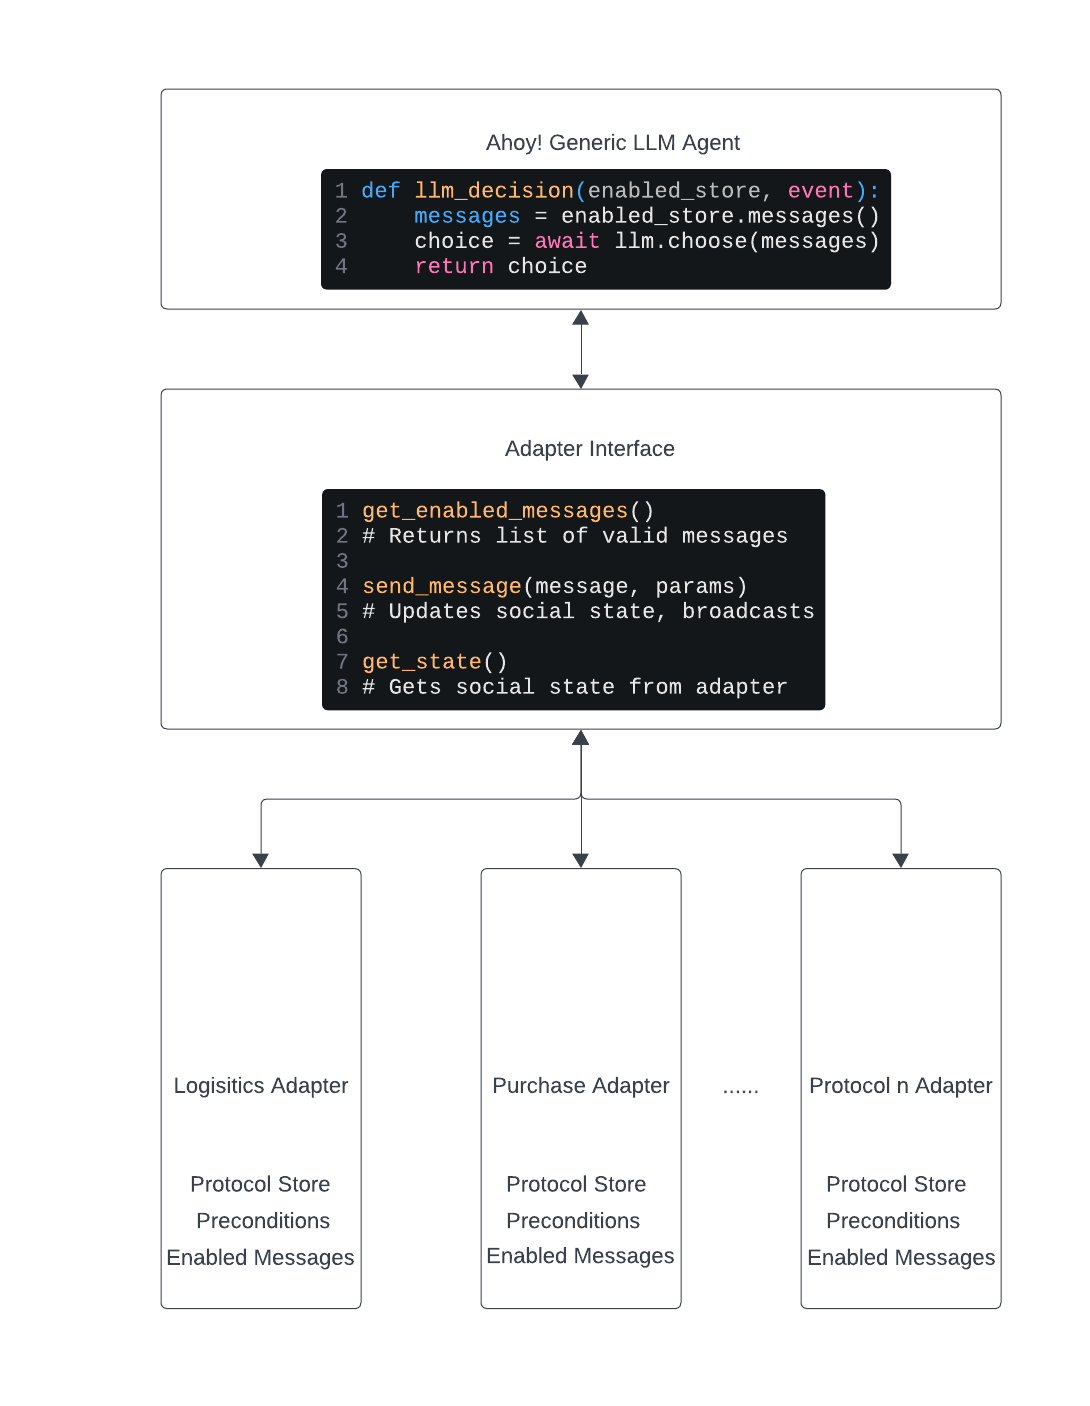
\includegraphics[width=\textwidth]{Images/Interface_Diagram.png}
%     \label{fig:interface_diagram}
% \end{figure*}

% \akc{one adapter per protocol and therefore isolation does not make sense to me.} 

% This approach offers the programmer the guarantees described in Table \ref{tab:guarantees}.
% \begin{table*}[ht]
%     \centering
%     \begin{tabular}{|c|c|c|}
%         \hline
%         & Guarantee & Description \\
%         \hline
%         1 & Protocol Correctness & Only valid messages are offered to the LLM.\\
%         2 & Parameter Scoping & Parameters from one protocol do not leak to another \\
%         3 & Role consistency & Only role-specific messages are offered to the LLM \\
%         4 & Termination & Protocols either reach a terminal state or deadlock is detected \akc{?}\\
%         5 & Auditablity & Execution trace is auditable and can be replayed \\
%         \hline
%     \end{tabular}
%     \caption{ChiPS {\ahoy} Framework Guarantees}
%     \label{tab:guarantees}
% \end{table*}
A key contribution of \ahoy is a programming model centered on the LLM decision endpoint pattern, which enables protocol-agnostic agent implementations.
This programming model can be used at three distinct levels of expertise.
At the \emph{user} level, end users interact with pre-configured agents and protocols through a dialog interface without writing any code.
At the \emph{protocol} level, domain experts can define new protocols and configure agents for these protocols using declarative syntax while writing minimal code.
At the \emph{framework} level, we provide support for developers to extend \ahoy by implementing custom event handlers, decision endpoints, or new LLM tooling.


\subsection{Level 1: End Users}
End users interact with \ahoy agents through the dialog interface.
No code knowledge is required.
Users can describe their goals in natural language (e.g, "I want to buy a pen and deliver it to [Address]") and \ahoy uses the LLM-based protocol and role selection module to map the user intent to the appropriate protocol and role, then launches the agent automatically.
This interface is provided by \ahoy: users do not need to understand protocols, adapters, or LLM endpoints.

\subsection{Level 2: Domain Experts}
Domain experts can define new protocols and configure agents for them using \ahoy.
This level also requires no python coding --- declarative BSPL syntax is sufficient.
Protocol developers:
\begin{enumerate}
    \item \textbf{Write Protocol Specifications:} Define roles, messages (with typed input and output parameters), and constraints in BSPL (see Section \ref{sec:Background}). For example, to add a new contract negotiation protocol, a domain expert writes the appropriate BSPL specification defining the Proposer and Acceptor roles, the messages they exchange, and the in/out parameters that govern message ordering.
    \item \textbf{Register Protocol Metadata:} Add a one--line protocol description to the appropriate file that can be read by \ahoy and serves as an input to the protocol and role selection module.
    \item \textbf{Configure Agent Behavior:} Specify agent goals and constraints in a human--readable input file (e.g, "Accept offers above \$$100$", "Propose at least a $10\%$ markup"). These constraints are provided to the LLM as part of the system prompt.
    \item \textbf{Test and Deploy:} \ahoy automatically handles protocol validation, adapter instantiation, and LLM integration. No code changes are required.
\end{enumerate}
In this manner, \ahoy enables domain experts to focus solely on the protocol structure and agent goals, without the need to handle any implementation details.

\subsection{Level 3: Framework Developers}
Developers can extend \ahoy by adding new tools for LLM use, custom events that can trigger an LLM call, or custom decision strategies that do not need LLM integration.
In order to modify \ahoy, developers need to understand the decision endpoint pattern shown in Listing \ref{lst:ahoy-dec}.

\begin{lstlisting}[language=Python, caption=Ahoy Decision Endpoint Pattern,label=lst:ahoy-dec]
from bspl.adapter import Adapter
from lib.state_manager import serialize_adapter_state
from lib.llm_client import AnthropicLLMClient

adapter = Adapter(Seller, systems, agents)
llm_client = AnthropicLLMClient()

async def llm_decision(enabled_store, event):
    # Serialize current protocol state
    state = serialize_adapter_state(adapter)
    
    # Get available messages from enabled_store
    enabled_messages = list(enabled_store.messages())
    
    # Delegate reasoning to LLM
    llm_response = await llm_client.complete(
        messages=[{
            "role": "user",
            "content": f"State: {state}. "
                      f"Enabled messages: {enabled_messages}. "
                      f"Goal: Choose action (price 10-100). "
                      f"What message to send?"
        }]
    )
    
    # Parse LLM response and bind parameters
    decision = parse_llm_response(llm_response)
    message_instance = bind_message(decision, enabled_store)
    
    return message_instance

# Register handler with decision endpoint
adapter.decision()(llm_decision)
\end{lstlisting}

%%%%%%%%%%%%%%%%%%%%%%%%%%%%%%%%%%%%%%%%%%%%%%%%%%%%%%%%%%%%%%%%%%%%%%%%%%%%%%%%%
\section{Demos}

% \subsection{Research Questions [TBD]}
% \begin{itemize}
%     \item[RQ1] {\ahoy} agents can execute multiple protocols with similar decision quality and efficiency, requiring no protocol-specific agent modifications.
%     \item[RQ2] Framework guarantees from Table \ref{tab:guarantees} hold across logistics and purchase protocols.
%     \item[RQ3] The protocol selection module achieves high accuracy for user intents mapped to available protocols.
% \end{itemize}

% \subsection{Experimental Design}
% \oj{couple of ideas I had for the experiments we can run for the workshop submission}
% \begin{itemize}
%     \item Protocol Detection Accuracy: Test the protocol selection module with ambiguous user inputs and measure the precision, accuracy and recall of protocol--role pair selection.
%     \item Guarantee Validation: Execute curated scenarios, record complete protocol enactment traces (message sequence, parameter bindings and protocol--specific information) and verify that all six framework guarantees from Table \ref{tab:guarantees}] are maintained
% \end{itemize}

Our experiments demonstrate three key capabilities of \ahoy:
\begin{enumerate}
    \item Protocol Portability: The same agent code executes correctly across different protocols without modification.
    \item Enforcement of Guarantees: Structural guarantees are maintained in all enactments.
    \item Protocol Selection Accuracy: The protocol selection module reliably maps user intent to appropriate protocols and roles.
\end{enumerate}

\subsection{Demo 1: Protocol Portability}
\textbf{Goal:} Demonstrate that a single \ahoy agent can enact multiple protocols without code changes.\\
\textbf{Method:} Execute identical agent decision logic in two distinct protocol contexts:
\begin{itemize}
    \item Purchase Protocol (Buyer role): Agent participates in a buyer--seller-shipper negotiation.
    \item Logistics Protocol (Merchant role): Agent coordinates packaging and shipping workflow.
\end{itemize}
Both enactments use the same underlying LLM decision endpoint pattern shown in Listing \ref{lst:ahoy-dec}.
No protocol--specific logical branches or conditional code paths are used.\\
\textbf{Results:} We capture execution traces from both protocols and verify the following.
\begin{itemize}
    \item Both protocols reach terminal state.
    \item Message sequences respect protocol--specific constraints.
    \item No adapter exceptions or schema violations occur.
    \item LLM decision quality is consistent across both domains. \oj{no stupid decisions}
\end{itemize}

\subsection{Demo 2: Guarantee Validation}
\textbf{Goal:} Verify that the framework guarantees hold across protocols.\\
\textbf{Method:} We execute curated scenarios targeting the core guarantees:
\begin{itemize}
    \item Message Validity: Verify that only schema--conforming messages are offered to the LLM.
    \item Parameter Scoping: Test scenarios where identical parameter names (e.g. orderID) appear in two or more protocols; verify that they remain isolated and do not contaminate across protocol contexts.
    \item Role Consistency: Confirm that only role--appropriate messages appear in the enabled message set at each decision point.
\end{itemize}
\textbf{Results:} We produce a trace validation report documenting:
\begin{itemize}
    \item Scenario description
    \item What would break in a naive agent
    \item How \ahoy handles it.
    \item Exceptions noted.
\end{itemize}

\subsection{Demo 3: Concurrent Multiprotocol Participation}
\textbf{Goal:} Demonstrate that a single LLM-driven agent can simultaneously participate in multiple protocol instances while maintaining state isolation and making coherent decisions across different protocol contexts.\\
\textbf{Method:} We instantiate parallel protocol enactments where the agent operates in distinct roles across multiple protocols concurrently:
\begin{itemize}
    \item \textbf{Scenario Setup:} Agent acts as Buyer in Purchase protocol while simultaneously acting as Merchant in Logistics protocol.
    \item \textbf{State Isolation:} Each protocol maintains an independent adapter with isolated social state (message history, parameter bindings, enabled messages).
    \item \textbf{Decision Interleaving:} We trigger decision events across both protocols in an interleaved fashion, simulating realistic concurrent coordination.
    \item \textbf{Context Switching:} The LLM receives distinct user prompts for each protocol, including protocol-specific enabled messages and agent goals, testing whether the LLM maintains context separation.
\end{itemize}
\textbf{Results:} We capture execution traces from both concurrent protocol enactments and verify:
\begin{itemize}
    \item \textbf{Parameter Isolation:} Parameters bound in one protocol (e.g., orderID in Purchase) do not interfere with identically-named parameters in another protocol (e.g., orderID in Logistics).
    \item \textbf{Message History Separation:} Each protocol's message history remains isolated; the LLM references only relevant messages when making decisions in each context.
    \item \textbf{Coherent Decision Making:} Decisions made in one protocol do not violate constraints or create contradictions in the other protocol.
    \item \textbf{No Cross-Protocol Contamination:} Enabled message sets correctly reflect only messages available in each specific protocol context.
    \item \textbf{Concurrent Termination:} Both protocols reach terminal state independently without deadlock or state corruption.
\end{itemize}

\subsection{Demo 4: Decision Quality Across Domains}
\textbf{Goal:} Show that the LLM reasoning adapts seamlessly and makes semantically appropriate choices in different protocol contexts.\\
\textbf{Method:} We capture decision point snapshots from representative protocol enactments:
\begin{itemize}
    \item Purchase Protocol: LLM chooses the appropriate price to buy items.
    \item Logistics Protocol: LLM chooses the appropriate material to wrap the package based on frailty without explicit guidance.
\end{itemize}
\textbf{Results:} Table showing
\begin{itemize}
    \item Scenario description
    \item LLM action and reasoning
    \item Semantic appropriateness of decision in context (LLM as judge?)
\end{itemize}

\subsection{Demo 5: Protocol Selection Accuracy}
\textbf{Goal:} Validate that the protocol selection module reliably maps user intent to correct protocol--role pairs.\\
\textbf{Method:} We construct a test set of $n$ user intent statements, including:
\begin{itemize}
    \item Clear Purchase Intents: I want to buy a notebook
    \item Clear Logistics Intents: I want to organize packaging and shipping for a warehouse containing the following items \ldots
    \item Ambiguous intent: I want to ship something
\end{itemize}
Each test case has a ground truth protocol label.\\
\textbf{Results:} A results table showing 
\begin{itemize}
    \item User input
    \item Ground truth label
    \item Difficulty marker
    \item Selection output
\end{itemize}
and a summary table showing the accuracy, recall and precision.

\subsection{Demo 6: Custom LLM Events}
\textbf{Goal:} Demonstrate that \ahoy agents can respond to both protocol-driven events (received messages) and custom business logic events (timeouts, thresholds, periodic checks) using the same LLM decision endpoint.\\
\textbf{Method:} We instantiate agents that handle concurrent event sources:
\begin{itemize}
    \item \textbf{Adapter Reactions:} Traditional protocol event handlers triggered when messages arrive.
    \item \textbf{Custom Events:} Business logic triggers such as periodic timeout checks, stall detection, or out-of-stock alerts.
    \item \textbf{Synchronization:} Both event paths converge on the same \texttt{choose\_and\_bind()} decision logic, synchronized via \texttt{asyncio.Lock} to prevent concurrent access conflicts.
\end{itemize}
Test scenarios include:
\begin{itemize}
    \item Purchase Protocol (Buyer with periodic timeout): Adapter processes incoming quotes; custom event handler gets a ping from a mocked inventory system after 30 seconds to buy a laptop.
    \end{itemize}
\textbf{Results:} We verify that:
\begin{itemize}
    \item \textbf{Concurrent Execution:} Both adapter and custom event paths execute without race conditions or deadlocks.
    \item \textbf{Unified Decision Logic:} Both event types use identical parameter-binding and message-sending workflows.
    \item \textbf{Constraint Preservation:} Messages from both paths respect protocol constraints and parameter bindings.
    \item \textbf{Metric Tracking:} LLM call counts correctly reflect decisions from both adapter and custom event handlers.
    \item \textbf{Graceful Termination:} Agents exit cleanly when protocols complete or thresholds are exceeded.
\end{itemize}

\subsection{Summary}
Together, these experiments demonstrate that \ahoy achieves protocol--agnosticism.
A single, generic agent implementation using \ahoy, correctly selects and enacts multiple protocols, fulfills all structural guarantees, and makes semantically sound decisions without protocol--specific code modifications.


%%%%%%%%%%%%%%%%%%%%%%%%%%%%%%%%%%%%%%%%%%%
\section{Related Work}
This section positions our work within the broader landscape of multiagent systems, LLMs and agent programming models.
\subsection{LLMs in Multiagent Systems}
Recent work explores the use of Large Language Models as reasoning engines in multiagent systems.
Key approaches for LLM interaction include:
\begin{itemize}
    \item In Context Learning
    \item Fine Tuning
    \item Chain of Thought Reasoning
\end{itemize}
In addition, there has been a push towards improving communication between LLM agents.
Various approaches define protocols and communication patterns that enable LLM-based agents to coordinate effectively.
Our work differs from existing approaches by focusing on \emph{dynamic protocol selection and enactment:} given user intent expressed in natural language dialog, our framework automatically selects from multiple available protocols and binds the agent to the appropriate role without requiring protocol--specific agent implementations.
\oj{Explain how we differ from each prompting approach}

\subsection{Programming Models}
Established programming models for multiagent systems include the Actor model, reactive agents and BDI (Belief--Desire--Intention) architectures.
These provide different abstractions for agent behavior and coordination.
Our \ahoy framework complements these by \ldots

\cite{singh2011information}
\bibliographystyle{splncs04}
\bibliography{Omkar}
\end{document}
